\section{المحول في الرؤية الحاسوبية}
في هذه الفقرة سنذكر استخدامات نموذج المحول في مجال الرؤية الصنعية، إذ بسبب النجاح الذي حققه المحول في تطبيقات معالجة اللغات الطبيعية، فقد استخدم في مجالات الرؤية الحاسوبية في السنوات الأخيرة، وقدأعطى نتائج تفوقت على أحدث وأفضل الخوارزميات في هذا المجال بالنسبة للعديد من معايير التقييم في هذا المجال مثل 
\textLR{Imagenet, coco}
وغيرها
\textLR{\cite{ViTsurvey}}.
فقد تم استخدام المحول في مجال توليد
\textLR{\cite{Transgan}}،
تصنيف
\textLR{\cite{ViT}}،
كشف
\textLR{\cite{DETR}}،
وتحسين الصور
\textLR{\cite{Pre-trainedimageTransformer}}،
تصنيف الفيديو
\textLR{\cite{Non-local neural networks}}،
والملاحقة
\textLR{\cite{transformertracker}}،
والذي هو موضوع بحثنا.
\newline
سنتكلم بإيجاز في هذه الفقرة عن النماذج الأولى والأساسية التي استخدمت المحول في مجال الرؤية الصنعية وهي نموذج
\textLR{ViT\cite{ViT}}
ونموذج
\textLR{DETR\cite{DETR}}.
وقد ظهرت بعدها الكثير من النماذج التي اعتمدت على المحول في تطبيقات الرؤية الحاسوبية.
\subsection{المحول والشبكات التلافيفية}
ذكرنا في فقرة سابقة 
\ref{section:transformer}
أن المحول استغنى عن شبكات 
\textLR{RNN}
والتي كانت الأكثر استخداما في مجال معالجة اللغات الطبيعية
\textLR{\cite{Vaswani17}}،
وتحدثنا عن المشكلات التي تعاني منها هذا النوع من الشبكات ذات المعالجة التسلسلية. أما فيما يخص الرؤية الحاسوبية فإن شبكات
\textLR{CNN}
هي الأكثر استخداماً، وهي على العكس من شبكات 
\textLR{RNN}
يمكن بفعالية أن تعالَج بشكل تفرعي باستخدام  
\textLR{GPU}.
ولكن حتى الآن فإن الكثير من الأبحاث لم تستبدل شبكات
\textLR{CNN}
بنموذج المحول بشكل كلي بالرغم من تفوق المحول في الأداء عند تدريبه على معطيات كافية. والسبب في ذلك يعود إلى محاسن شبكات 
\textLR{CNN}
من حيث المحلية
\textLR{locality}،
أي أخد البكسلات المجاورة بعين الاعتبار عند المعالجة كما سنذكر لاحقاً.
\subsubsection{ميزات الشبكات التلافيفية}
\begin{itemize}
\item
غير متغيرة مع الانسحاب
\item
تأخذ العمليات الحسابية في هذه الشبكات المناطق المحلية بعين الاعتبار، فبالتالي السمات المستخرجة منها حساسة محلياً وتحمل معلومات مكانية بشكل أكبر من المحول.
\item
وبسبب هذه الميزة وهي المحلية،
فإن
\textLR{CNN}
جيدة لاستخراج السمات من الصورة، ولكن ليست قادرة على نمذجة العلاقات أو الارتباطات بين هذه السمات، وبالتالي تفتقر إلى الفهم العام للصورة. أما بالنسبة للمحول فإن نقطة قوته هي القدرة على فهم السياق العام
\textLR{\cite{TransformerCV}}،
والنمذجة بشكل
\textLR{global}
أي نمذجة العلاقات الطويلة الأمد بين السمات
\textLR{long-range dependencies}
\textLR{\cite{Swin Transformer V1 and V2}}.
\end{itemize}
بعض الأعمال استخدمت المحول في مجال الرؤية الحاسوبية وقد أعطت نتائج تفوقت على الخوارزميات الرائدة في هذا المجال عند وجود عدد كافي من معطيات التدريب، وذلك بالاعتماد فقط على توابع الانتباه ودون أي استخدام للشبكات التلافيفية 
\textLR{\cite{ViT}}،
بالرغم من أن هذه النماذج لها بنية أبسط، وتستهلك زمن تدريب أقل مقارنة بنماذج الشبكات التلافيفية
\textLR{\cite{TransformerCV}}.
\subsection{المحول في مجال التصنيف}
ظهرت العديد من خوارزميات التصنيف التي تستخدم المحول في السنوات الأخيرة، بعضها قد حسن الخوارزميات المعتمدة على الشبكات التلافيفية بإضافة أجزاء من المحول إليها، وذلك كونه ينمذج الترابطات الطويلة الأمد، مثل
\textLR{VT\cite{VT}}،
\textLR{BotNet\cite{BotNet}}.
وكون البنية الأصلية للمحول 
\textLR{\cite{Vaswani17}}
تهمل المعلومات المحلية، لذلك كان هنالك العديد من التحسينات على بنية
\textLR{ViT\cite{ViT}}،
من هذه التحسينات إضافة أجزاء من الشبكات التلافيفية لتحسين المحول، مثل خوارزمية
\textLR{BEiT\cite{BEiT}}،
وخوارزمية 
\textLR{ConViT\cite{ConViT}}.
\newline
وهناك تحسينات أخرى مثل المحول الذي يعتمد على الانتباه المحلي،
هذه الخوارزميات قد أعادت تصميم تجزئة الصورة 
\textLR{patch partition}،
وأعادت تصميم كتل توابع الانتباه بهدف إضافة المعلومات المحلية(المكانية) إلى المحول، دون الاعتماد على الشبكات التلافيفية وذلك مثل خوارزمية 
\textLR{TNT\cite{TNT}}،
\textLR{Volo\cite{Volo}},
و 
\textLR{SwinTransformer\cite{swintransformer}}
والتي سنتحدث عنها في الفقرة
\ref{section:swinTransformer}
كونها الـ
\textLR{backbone}
المستخدم في نموذجنا.
\newline
عدلت العديد من الأبحاث بنية المحول  إلى بنية هرمية وعميقة مثل
\textLR{T2T-ViT\cite{T2T-ViT}}،
\textLR{PVT\cite{PVT}}،
وذلك محاكاة لبنية الشبكات التلافيفية الهرمية والعميقة 
\textLR{\cite{Why Deep Learning Works}}.
\newline
بحسب المقالة
\textLR{\cite{ViTsurvey}}،
والتي تقارن وتصنف أكثر من مئة محول في مجال الرؤية الحاسوبية فإن الأبحاث الحديثة لا تميل إلى استخدام البنية الأصلية للمحول، ولم تستغني عن استخدام الشبكات التلافيفية بشكل كامل، بل العكس من ذلك استخدام البنية الهجينة هو ما يعطي أفضل النتائج، بالرغم من أن المحول يمكن أن يوازي بأداءه الشبكات التلافيفية أو حتى يفوقها في الأداء، ويعود ذلك إلى أن المعلومات المحلية مهمة جداً لتحسين أداء المحول كما في 
\textLR{Volo\cite{Volo}}،
و
\textLR{SwinTransformer\cite{swintransformer}}،
وهما نسخة المحول الأكثر استخداما في الرؤية الحاسوبية.
في هاتين الخوارزميتين تم استخدام خليط من المعلومات العامة 
\textLR{global}
والمعلومات المحلية 
\textLR{local}.
\newline
أما على صعيد تحسين الاجزاء الأخرى من المحول مثل تحسين الترميز المكاني
\textLR{Positional Encoding PE}
فهناك العديد من الأبحاث مثل
\textLR{\cite{Conditional positional encodings for ViT}}،\textLR{\cite{RethinkingPE}}،\textLR{\cite{deeper look at position information in cnns}}. 
أو تحسين بنية
\textLR{MHA}
الانتباه متعدد الرؤوس
\textLR{\cite{Cordonnier}}،
أو تحسين 
\textLR{MLP}
كما في 
\textLR{\cite{Attention is not all you need}}.
\subsection{المحول في مجال الكشف}
أول خوارزمية استخدمت المحول في مجال الكشف هي 
\textLR{DETR\cite{DETR}}،
استخدمت هذه الخوارزمية تمثيل جديد وهو
\textLR{object query}،
وهو أحد مداخل مفكك الترميز،
وهو مجموعة من الأوزان القابلة لتعلم السمات العامة في الصورة. كان هناك العديد من التحسينات على هذه الخوارزمية مثل
\textLR{DeformableDETR\cite{DeformableDETR}}،
و
\textLR{ACT\cite{ACT}}،
كون الخوارزمية الأصلية
\textLR{\cite{DETR}}
تعاني من دقة كشف منخفضة من أجل الأغراض الصغيرة وتأخذ زمن طويل في التدريب.
\newline
هناك العديد من الدراسات التي أعادت تصميم بنية المحول مثل
\textLR{TSP\cite{TSP}},
\textLR{YOLOS\cite{YOLOS}}.
أو باستخدام المحول كـ
\textLR{backbone}
لاستخلاص السمات من الصورة كما في
\textLR{FPT\cite{FPT}}.
\subsection{خوارزمية التصنيف
\textLR{ViT\cite{ViT}}}
هذه الخوارزمية لا تستخدم الشبكات التلافيفية في بنيتها. إذ يتم تقسيم الصورة إلى أقسام عدة
\textLR{patches}،
كل قسم
\textLR{patch}
يعامل معاملة ال 
\textLR{token}
(الكلمة) في المحول الأصلي، أي يتم إدخاله إلى طبقة
\textLR{embedding}
خطية لتحويله إلى شعاع بأبعاد مختلفة.
\newline
عند تدريب هذا النموذج على معطيات تدريب ذات حجم متوسط مثل
\textLR{ImageNet}
كان أداؤه متواضع وأقل من أداء نموذج
\textLR{ResNet\cite{ResNet}}
و بعدد أوزان متقارب. لكن النتائج تغيرت عند تدريبه على معطيات تدريب بحجوم كبيرة ( 
$14$
مليون -
$300$ 
مليون عينة) مثل 
\textLR{ImageNet-21K},
\textLR{JFT-300M}،
عندها أعطى النموذج نتائج تفوقت على الخوارزميات السابقة.
\newline
دخل النموذج الأصلي للمحول هو سلسلة ببعد واحد . للتعامل مع الصورة وللمحافظة على البنية الأساسية للمحول فقد  تم تعديل الصورة
$x\in \mathds{R}^{H\mathsf{x}W\mathsf{x}C}$
وتحويلها إلى سلسلة من الأجزاء المسطحة
$x_p \in  \mathds{R}^{N\mathsf{x}(P^2.C)}$
ذات بعد واحد، وذلك لمحاكاة دخل المحول الأصلي. حيث
$H\mathsf{x}W$
أبعاد الصورة،
$C$
عدد القنوات والتي هي في الغالب
$RGB = 3$،
$P\mathsf{x}P$
أبعاد كل قسم من الصورة
\textLR{patch}،
$N$
 عدد الأقسام أو الأجزاء
$N = \frac{HW}{P^2}$.
\newline
يتم إدخال الشعاع 
$x_p$
إلى طبقة إسقاط خطي أي شبكة عصبونية بطبقة واحدة مع تابع تفعيل خطي، وذلك لتحويل أبعاده إلى 
$(N,D)$
كما في المعادلة
\ref{eq:vit1}.
\begin{equation}
z_0 = [x_{class};X_p^1E;x_p^2E;...;x_p^NE]+E_{pos},	E\in \mathds{R}^{(P^2.C)\mathsf{x}D},E_{pos}\in \mathds{R}^{(N+1)\mathsf{x}D}
\label{eq:vit1}
\end{equation}
\begin{equation}
Z_l^\prime = MSA(LN(z_{l-1})) + z_{l-1},	l = 1 ... L
\label{eq:vit2}
\end{equation}
\begin{equation}
Z_l = MLP(LN(z_l^\prime)) + z_l^\prime,	l = 1 ... L
\label{eq:vit3}
\end{equation}
\begin{equation}
y = LN(z_L^0)
\label{eq:vit4}
\end{equation}
حيث
$D$
هو
\textLR{hyperparameter}
ويمكن تسميته ببعد الـ
\textLR{embedding}.
$E$
هي طبقة الإسقاط الخطي، بعدد بارامترات
$E \in \mathds{R}^{(P^2.C)\mathsf{x}D}$
قابلة للتدريب.
وكما في خوارزمية
\textLR{BERT\cite{BERT}}
فيتم إضافة شعاع من البارامترات ندعوه بالـ
\textLR{class token}
قابل للتدريب بأبعاد
$(1\mathsf{x}D)$،
وهو 
$x_{class}$
في المعادلة 
\ref{eq:vit1}.
 حيث يتم اعتبار أن حالة هذا الشعاع في الخرج النهائي للمحول
$z_L^0$
يمكن تدريبها لتعبر عن صنف الصورة، وذلك بعد تعديل هذا الشعاع بإدخاله إلى شبكة التصنيف
\textLR{classification head}.
$L$
هي عدد طبقات المرمز.
\newline
نضيف إلى هذا الشعاع شعاع ترميز الموقع 
$E_{pos}$
وذلك لإدخال المعلومات المكانية النسبية بين أجزاء الصورة، استخدمت
\textLR{ViT}
ترميز موقع ببعد واحد قياسي.
$Z_0$
هو دخل المحول كما في المعادلة
\ref{eq:vit1}.
\newline
يستخدم
\textLR{ViT}
بنية مرمز مطابقة لبنية المرمز في المحول الأصلي من حيث توابع انتباه متعددة الرؤوس كما في المعادلة 
\ref{eq:vit2}
وشبكة
\textLR{MLP}
كما في المعادلة 
\ref{eq:vit3},
ويتم تطبيق طبقة تقييس قبل كل كتلة، بالإضافة إلى 
\textLR{residual connections\cite{residual}}
بعد كل كتلة. وكما يوضح الشكل
\ref{fig:ViT}

\begin{figure}[h!]
	\centerline{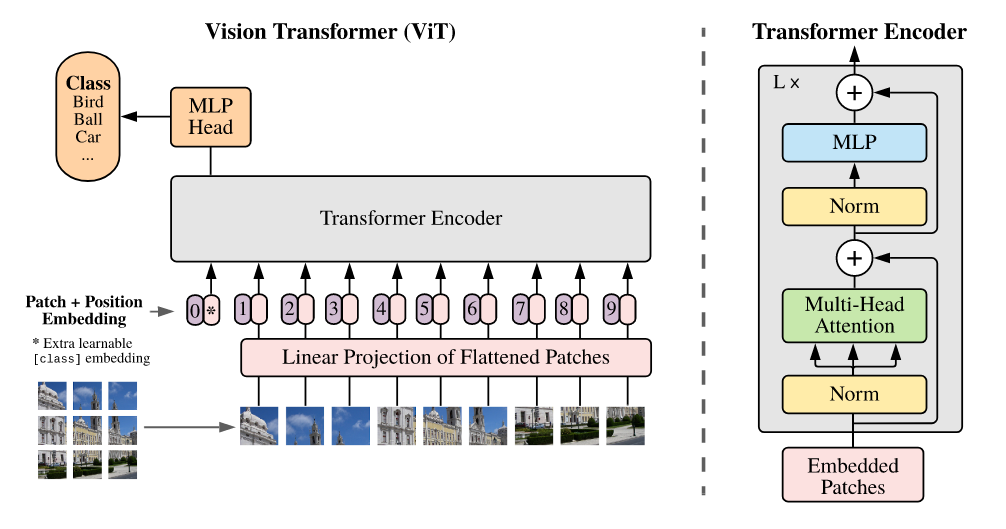
\includegraphics[width=\textwidth]{images/ViT}}
	\caption{
	\textRL{بنية خوارزمية}
	\textLR{ViT}
	\textLR{\cite{ViT}}}
	\label{fig:ViT}
\end{figure}

\subsection{خوارزمية الكشف
	\textLR{DETR\cite{DETR}}
\label{section:detr}}

\begin{figure}[h!]
	\centerline{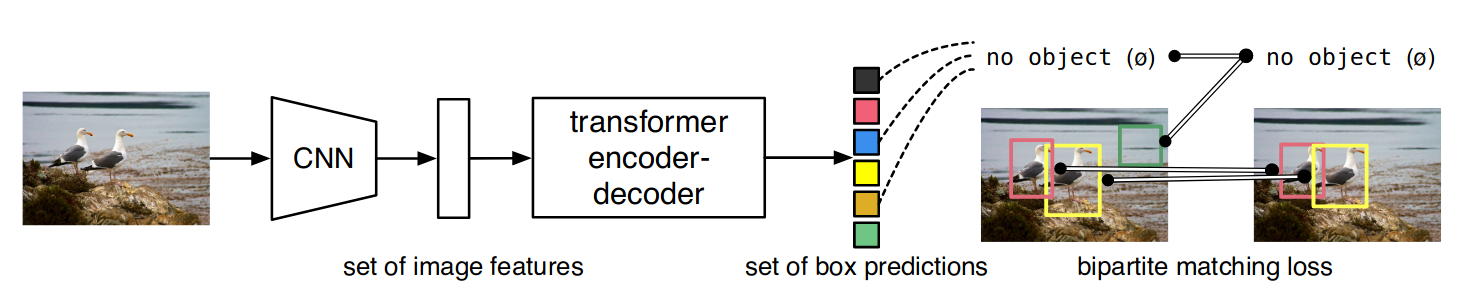
\includegraphics[width=\textwidth]{images/DETR}}
	\caption{\textRL{بنية الكاشف}
	\textLR{DETR}
	\textLR{\cite{DETR}}}
	\label{fig:DETR}
\end{figure}
\selectlanguage{arabic}
كما يوضح الشكل
\ref{fig:DETR}
فإن النموذج يستخدم شبكة تلافيفية كـ
\textLR{backbone}
 لاستخلاص السمات من الصورة التي أبعادها
$x_{img} = \in \mathds{R}^{3\mathsf{x}H_0\mathsf{x}W_0}$،
وأبعاد خريطة السمات بعد الشبكة التلافيفية
$f \in \mathds{R}^{C\mathsf{x}H\mathsf{x}W}$،
حيث
$H,W = \frac{H_0}{32},\frac{W_0}{32}$
و
$C = 2048$.
يتم تخفيض الأبعاد من $C$ إلى  $d$، وتحويل خريطة السمات من بعدين إلى بعد واحد عبر التسطيح
\textLR{flattening}
 فيصبح لدينا أبعاد دخل المرمز
$N\mathsf{x}d$
حيث
$N=H\mathsf{x}W$.
\newline
ونلاحظ أيضا أن الخوارزمية قد اتبعت بنية المحول الأصلي أي بنية مرمز-مفكك ترميز مع فوارق بسيطة مثل دخل مفكك الترميز. في  المحول الأصلي دخل مفكك الترميز هو الخرج في اللحظة الزمنية السابقة، أما في 
\textLR{DETR} 
فهو عبارة بارامترات قابلة للتدريب تدعى
\textLR{object queries}،
تعبر عن ترميز مكاني لكل غرض ويتم فك هذا الترميز عبر مفكك الترميز.
نلاحظ أن كل من الخوارزميتين السابقتين 
\textLR{ViT}
و
\textLR{DETR}
استخدمتا بنية المحول الأصلي مع تعديلات بسيطة. أما بالنسبة  للخوارزمية التي استخدمناها لاستخلاص السمات في نموذجنا وهي محول
\textLR{Swin\cite{swintransformer}}،
والتي سنتحدث عنها في الفقرة التالية فقد عدلت بشكل كبير في بنية المحول.
